%%%%%%%%%%%%%%%%%%%%%%%%%%%%%%%%%%%%%%%%%
% Beamer Presentation
% LaTeX Template
% Version 1.0 (10/11/12)
%
% This template has been downloaded from:
% http://www.LaTeXTemplates.com
%
% License:
% CC BY-NC-SA 3.0 (http://creativecommons.org/licenses/by-nc-sa/3.0/)
%
%%%%%%%%%%%%%%%%%%%%%%%%%%%%%%%%%%%%%%%%%

%----------------------------------------------------------------------------------------
%	PACKAGES AND THEMES
%----------------------------------------------------------------------------------------

\documentclass{beamer}

\mode<presentation> {

% The Beamer class comes with a number of default slide themes
% which change the colors and layouts of slides. Below this is a list
% of all the themes, uncomment each in turn to see what they look like.

%\usetheme{default}
%\usetheme{AnnArbor}
%\usetheme{Antibes}
%\usetheme{Bergen}
%\usetheme{Berkeley}
%\usetheme{Berlin}
%\usetheme{Boadilla}
%\usetheme{CambridgeUS}
%\usetheme{Copenhagen}
%\usetheme{Darmstadt}
%\usetheme{Dresden}
%\usetheme{Frankfurt}
%\usetheme{Goettingen}
%\usetheme{Hannover}
%\usetheme{Ilmenau}
%\usetheme{JuanLesPins}
%\usetheme{Luebeck}
\usetheme{Madrid}
%\usetheme{Malmoe}
%\usetheme{Marburg}
%\usetheme{Montpellier}
%\usetheme{PaloAlto}
%\usetheme{Pittsburgh}
%\usetheme{Rochester}
%\usetheme{Singapore}
%\usetheme{Szeged}
%\usetheme{Warsaw}

% As well as themes, the Beamer class has a number of color themes
% for any slide theme. Uncomment each of these in turn to see how it
% changes the colors of your current slide theme.

%\usecolortheme{albatross}
%\usecolortheme{beaver}
%\usecolortheme{beetle}
%\usecolortheme{crane}
%\usecolortheme{dolphin}
%\usecolortheme{dove}
%\usecolortheme{fly}
%\usecolortheme{lily}
%\usecolortheme{orchid}
%\usecolortheme{rose}
%\usecolortheme{seagull}
%\usecolortheme{seahorse}
%\usecolortheme{whale}
%\usecolortheme{wolverine}

%\setbeamertemplate{footline} % To remove the footer line in all slides uncomment this line
%\setbeamertemplate{footline}[page number] % To replace the footer line in all slides with a simple slide count uncomment this line

%\setbeamertemplate{navigation symbols}{} % To remove the navigation symbols from the bottom of all slides uncomment this line
}

\usepackage{graphicx} % Allows including images
\usepackage{booktabs} % Allows the use of \toprule, \midrule and \bottomrule in tables
\usepackage{listings}
\usepackage{amsmath}
\usepackage{algpseudocode,algorithm,algorithmicx}

\lstdefinestyle{customjava}{
  breaklines=true,
  frame=L,
  xleftmargin=\parindent,
  language=Java,
  showstringspaces=false,
  basicstyle=\footnotesize\ttfamily,
  keywordstyle=\bfseries\color{green!40!black},
  commentstyle=\itshape\color{gray!40!black},
  identifierstyle=\color{blue},
  stringstyle=\color{orange},
}

\lstdefinestyle{customcpp}{
  breaklines=true,
  frame=L,
  xleftmargin=\parindent,
  language=C++,
  showstringspaces=false,
  basicstyle=\footnotesize\ttfamily,
  keywordstyle=\bfseries\color{green!40!black},
  commentstyle=\itshape\color{gray!40!black},
  identifierstyle=\color{blue},
  stringstyle=\color{orange},
}
%----------------------------------------------------------------------------------------
%	TITLE PAGE
%----------------------------------------------------------------------------------------

\title[Interprocess Communication]{Interprocess Communication} % The short title appears at the bottom of every slide, the full title is only on the title page

\author{Jonathan Windle} % Your name
\institute[UEA] % Your institution as it will appear on the bottom of every slide, may be shorthand to save space
{
University of East Anglia \\ % Your institution for the title page
\medskip
\textit{J.Windle@uea.ac.uk} % Your email address
}
\date{\today} % Date, can be changed to a custom date

\begin{document}

\begin{frame}
\titlepage % Print the title page as the first slide
\end{frame}

\begin{frame}[allowframebreaks]
\frametitle{Overview} % Table of contents slide, comment this block out to remove it
\tableofcontents % Throughout your presentation, if you choose to use \section{} and \subsection{} commands, these will automatically be printed on this slide as an overview of your presentation
\end{frame}

%-------------------------------------------------------------------
\section{Cooperating Processes}
\begin{frame}
\frametitle{Cooperating Processes}
\begin{itemize}
\item Processes may either be:
\begin{itemize}
\item Independant
\item Cooperating
\end{itemize}
\item Cooperating processes need an interprocess communication mechanism to exchange data
\begin{itemize}
\item Shared memory
\item Message passing (i.e. signals)
\end{itemize}
\end{itemize}
\end{frame}
%-------------------------------------------------------------------
\section{Shared Memory IPC}
\begin{frame}
\frametitle{Shared Memory IPC}
\begin{itemize}
\item IPC using shared memory requires communicating processes to establish a region of shared memory
\item Typically this resides in the address space of the process creating the sshared memory segment
\item Processes are normally only able to access their own memory segment so this restriction must be relaxed.
\end{itemize}
\end{frame}
%--------------------------------------------------------------------
\section{Critical Sections}
\begin{frame}
\frametitle{Critical Sections}
\begin{itemize}
\item To avoid race conditions the key is to find some way to prohibit more than one process from reading and writing the shared data at the same time i.e. we need mutual exclusion.
\item Mutual Exclusion can be defined as some way of making sure that if one process is using the shared variable or file, the other process will be excluded from doing the same thing.
\item If we arranged matters so that no two processes were ever in their critical sections at the same time, ,we could avoid a race condition.
\item A solution must satisfy:
\begin{enumerate}
\item Mutual exclusion (No two must be in their critical section)
\item Progress: No process running outside its critical section may block another process.
\item Bounded Waiting: No process should have to wait forever to enter its critical section.
\end{enumerate}
\end{itemize}
\end{frame}
%--------------------------------------------------------------------------
\subsection{Guaranteeing Mutual Exclusion}
\begin{frame}
\frametitle{Guaranteeing Mutual Exclusion}
\begin{itemize}
\item The simplest solution is to have each process disable ALL interupts just after entering the critical section,and re-enable them just before leaving it.
\begin{itemize}
\item Since a process can only be switched as the result of an interrupt the CPU cannot be switched to another process.
\item But this approach is unnatractive, since it is generally unwise to give processes the power to turn off interrupts.
\end{itemize}
\item Initially, a single shares lock variable might appear to be a good idea but since it's a shared variable it's also susceptible to races.
\end{itemize}
\end{frame}
%------------------------------------------------------------------
\subsection{Coroutines}
\begin{frame}
\frametitle{Coroutines}
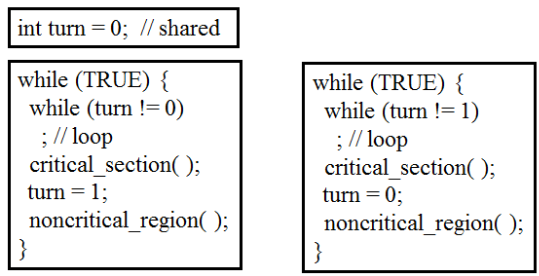
\includegraphics[scale=0.35]{coroute.png}
\begin{itemize}
\item Mutual exclusion is guaranteed, but:
\begin{itemize}
\item The processes must alternately access their critical sessions
\item If a process fails then the other process is hopelessly deadlocked i.e. the solution violates the no process outside the critical section can block another process.
\end{itemize}
\end{itemize}
\end{frame}
%--------------------------------------------------------------------
\subsection{Software Semaphores}
\begin{frame}
\frametitle{Software Semaphores}
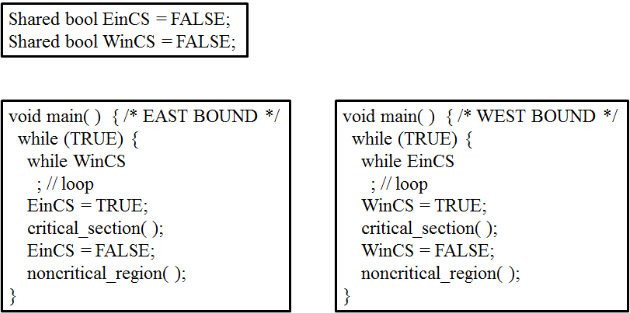
\includegraphics[scale=0.35]{sem1.png}
\begin{itemize}
\item Overcomes problem of lockstep synchronization
\item Program does not satisfy requirement for mutual exclusion:
\begin{itemize}
\item East want CS and steps over while test
\item Assume East is unloaded from CPU and replaced by West
\item West wants CS and can enter CS because EinCS is still false.
\end{itemize}
\end{itemize}
\end{frame}
%-----------------------------------------------------------------
\subsubsection{Software Semaphores - Fix}
\begin{frame}
\frametitle{Semaphores - Fixed}
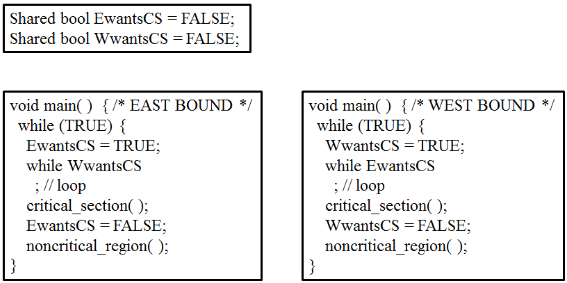
\includegraphics[scale=0.35]{sem2.png}
\begin{itemize}
\item Indicate desire to enter CS
\item If EnterCS check passes, assume OK to proceed.
\item Leads to deadlock... Let's hope semaphores don't come up... :D 
\end{itemize}
\end{frame}
%-----------------------------------------------------------------
\subsection{Hardware Support}
\begin{frame}
\frametitle{Hardware Support}
\begin{itemize}
\item The difficulty in software solutions for mutual exclusion was created by random interleaving of read and writes to memory
\item If the process was unloaded from the CPU between the read and write instructions then we cannot guarantee mutual exclusion
\item The problem can be eliminated if the hardware provides a memory access mechanism that allows the process to read a shared memory location, test it, and optionally change the value stored (depending on the result of the test)
\begin{itemize}
\item These operations must be performed indivisibly within one instruction (bus cycle)
\item The instruction is called a \texttt{Test-and-Set-Lock} (TSL) or \texttt{Read-Modify-Write} (RMW).
\end{itemize}
\end{itemize}
\end{frame}
%-------------------------------------------------------------------
\section{Test-and-Set-Lock}
\begin{frame}
\frametitle{Test-and-Set-Lock}
\begin{itemize}
\item Many computers, especially those designed with multiple processors have a TSL instruction:
\begin{itemize}
\item Syntax: TSL RX, LOCK; // RX = CPU register, LOCK = Memory location
\end{itemize}
\item TSL reads the contents of the memory word LOCK into register RX and then stores a non-zero value at the memory address LOCK.
\begin{itemize}
\item A key feature of the execution odTSL is that it locks the memory bus to prohibit other CPIs from aaccessing memory until it is done.
\item This also prevents the OS from unloading the process executing a TSL until it is done.
\item That is as one atomic, uninterruptable unit.
\end{itemize}
\end{itemize}
\end{frame}

%-----------------------------------------------------------------
\subsection{Using TSL}
\begin{frame}
\frametitle{Using TSL}
\begin{itemize}
\item We can use TSL to prevent two processes from simultaneously entering their critcal sections by implementing a simple LOCK.
\item A process sets the LOCK before executing its critical section and releases the LOCK when it has left the critical section.
\end{itemize}
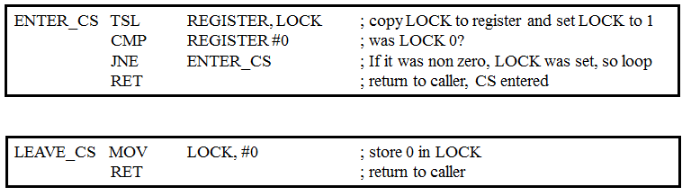
\includegraphics[scale=0.4]{tsl.png}
\end{frame}
%-----------------------------------------------------------------
\subsection{TSL-Summary}
\begin{frame}
\frametitle{TSL-Summary}
\begin{itemize}
\item The TSL instruction makes the solution to the critical section problem straightforward.
\begin{itemize}
\item Process must call \texttt{ENTER\_CS} and \texttt{LEAVE\_CS} at appropriate times for the solution to work.
\end{itemize}
\item There are some problems:
\begin{itemize}
\item One process might block another indefinitely
\item The proces waits ina busy-wait loop (wastes CPU cycles)
\item Extending to N processes?
\end{itemize}
\end{itemize}
\end{frame}
%---------------------------------------------------------------
\section{Summary}
\begin{frame}
\frametitle{Summary}
\begin{itemize}
\item Solutions to shared memory IPC use semaphores
\item Two types of Semaphore
\item General Semaphore:
\begin{itemize}
\item Can take any non-negative integer value, often called a counting semaphore
\item Useful if a number of processes need access to a resource
\end{itemize}
\item Binary Semaphore:
\begin{itemize}
\item Value can either be 1 or 0
\item Often called a mutex (as used to enforce mutual exclusion)
\end{itemize}
\item Solution:
\begin{itemize}
\item Acccess shared variables withing critical section and ensure access to critical sections are atomic.
\item Software solution: Dekkers
\item Hardware solution: TSL/RMW instructions.
\end{itemize}
\end{itemize}
\end{frame}
%------------------------------------------------------------------

\begin{frame} 
\Huge{\centerline{The End}}
\end{frame}

\end{document}